\documentclass{mcmthesis}
\mcmsetup{tcn = 0067 ,  problem = B, 
        sheet = true, titleinsheet =true, keywordsinsheet = true,
        titlepage = true, abstract = true}
\usepackage{palatino}
\usepackage{mwe}
\makeatletter
\newcommand{\figcaption}{\def\@captype{figure}\caption}
\newcommand{\tabcaption}{\def\@captype{table}\caption}
\makeatother
\usepackage{bm}
\usepackage{indentfirst}
\usepackage{booktabs}
\usepackage{longtable}
\usepackage{array} 
\setlength{\extrarowheight}{1.5pt}
\usepackage{mathpazo}
\usepackage{pgfplots}
\newcommand{\num}{pi}

\makeatletter
\def\@cite#1#2{\textsuperscript{[{#1\if@tempswa , #2\fi}]}}
\makeatother

\pgfplotsset{compat=1.8}
 % define the plot style and the axis style
\tikzset{elegant/.style={smooth,thick,samples=50,magenta}}
 % define the binom function
\tikzset{declare function={
            binom(\k,\n,\p)=\n!/(\k!*(\n-\k)!)*\p^\k*(1-\p)^(\n-\k);
            }
        }


\title{Cream of The Crop----Looking for The Best All Time College Coach}  %%title of this article

\date{\today}
\begin{document}
\begin{abstract}
\par After mathematically analyzing the question of selecting the  "best all time college coach",our modeling group would like to present our conclusions,strategies , and recommendations.

\par In the model of subjective judgement , we use the grey relational analysis model based on entropy weight method.we have define correlation degree  and determined the weights of their significance.By searching and selecting needed data , we obtained the final amount of evaluation of each coach in a certain sport.Finally , we compared the evaluation amounts and listed top five coaches , which is accordant with widely accepted result.Further work of the first  model , we ought to gather more data and set more evaluation factors.Only in this way , can we rank coaches in a more fairly way.
\par In the model of objective judgement , we adopt  the analytic hierarchy process to calculate the evaluation indexes. The algorithm offers us a convenient way to evaluate the excellence of certain coach , without any need for detailed information.After constructing the hierarchy and pairwise comparing the criteria with respect to the goal , we can obtain an rough ranking list , which need a mass of adjustment later.Through adjustment of proportion coefficient , we finally gain satisfactory results.This method can be applied to any time period and any ranking filed , because of its good applicability.
\par Taking the subjectivity of ranking of the coaches into account  ,  we will combine the results of the two models above in a certain proportion. The final results have quantities of  bias because of  the evaluation of individual things shall be avoided to the extent feasible.After testing a variety of real  data , we believe that the model is reliable.Furthermore , by slightly adjusting the coefficients , we can apply this model into various ranking field of sports.
\begin{keywords}
AHP; GRAP;Dual Model Fusion;Perfect Time-applicability;
\end{keywords}
\end{abstract}
\maketitle





\section{Introduction}   

\par In sports ,  a coach is a person involved in the direction ,  instruction and training of the operations of a sports team or of individual sportspeople. In college , a coach may also be a teacher.For most athletes involved ,  their coach is an influential element of the competitive experience. The Sport in America survey found that coaches are a leading positive\cite{1} influence on today's youth. Respondents were asked to rate the overall influence of a variety of groups on young people. Across all major demographic groups ,  coaches rank as the number one positive influence on youth today.
\par At their best ,  coaches can help their players improve their skills ,  perform to their best ability ,  develop strong character ,  and gain confidence. That is ,  they can maximize the positive value of sport ,  and they can enhance the intrinsic motivation to play sport. The intrinsic values of sport and the experience of mastery are more likely to generate fair play and good sportsmanship.
\par Therefore ,  it is necessary to build a model to evaluate the performance and achievement of coaches , In particular ,  the college coaches. Thus ,  it would be much easier for us to honor the best all time college coach.Moreover , coaches listed would be the good role models to emulate for the other coaches. 


\section{Problem Restatement and Analysis} 
\par On the one hand , according to the given question , we are required to build a comprehensive , hierarchical , have wide range of application and well time-applicability model to look for the "best all time college coach" male or female for the previous century.
\par On the other hand , we need to write an article using plain language for readers of this Sports Illustrated magazine , which should explain our selection criteria and the aspects of judgement.
\par Having considered about all the requirements above ,  our goal is to construct  a comprehensive evaluation model to select the best college coach statistically  , meanwhile ,  gain further analysis and answers for the problem. 




\section{Basic Assumptions} 
\begin{itemize}
\item Evaluation of the coach's coaching level ,  we take the coach's official games as the main part of the standard (taking MCAA data as the standard).A variety of friendly ,  warm-up match will not be considered.
\item Evaluation of the popularity of the coach, only consider Google search volume, the proportion of negative search volume will be included in consideration.Assuming Google clicks can reflect the prestige of coaches.
\item It is assumed that the rules of sports competitions do not change with time, and the intensity of competition does not change with time too.
\item Only using the data of Division one.
\item Assuming that the data we have chosen is true and reliable.
\item Assuming that coaches do not interact with each other.
\item Assuming the existing six evaluation indicators have been able to assess the level of the coach.
\end{itemize}

\par Under the basic assumptions, the analytic hierarchy process method and the multiplex model can be designed later.




\section{Symbol Description} 
\par In the section, we define some symbols when constructing the model as follows.
\begin{table}[h]
\centering
 \caption{\label{tab:test}Symbols Definition}
 \begin{tabular}{cc}
  \toprule
 Symbols & Definition  \\
  \midrule
$X=$&Objective judgement matrix  \\
$n , m$ &The number of coaches and judgement elements  \\
${E}_{1} , {E}_{2} ,..., {E}_{k}$ &The information entropy of each index \\
${W}_{j}$&The weight of each index\\
${X}_{0}$&     Reference data column\\
${\Delta }_{i}(j)$& The absolute difference\\
$a , b $& The intermediate variables\\
${y}_{i}$& Correlation coefficient\\
${r}_{i} $&Correlation degree\\
$CI$&  Coincidence indicator\\
$C$ &Coincidence ratio\\
$W$&  Corresponding feature vector\\\
$A$&Subjective judgement matrix  \\
${\lambda }_{max}$ & maximum eigenvalue of~$A$~\\
$S$&The final score\\
${P}_{t}$&The strength of competition \\
$\alpha $ &Subjective coefficient\\
$\beta $ & Objective coefficient\\
  \bottomrule
 \end{tabular}
\end{table}

\section{Model Preparation} 
\par Taking the evaluation of a coach into account  ,  we need to analyze this problem from the objective aspect and subjective aspect. However ,  there is no suitable single model to analyze these two aspects at the same time ,  so we need to establish an evaluation model combined with subjective and objective. After consulting the relevant information and choosing  ,  we use the Analytic Hierarchy Process (AHP) model to evaluate the coaches from the subjective aspect ,  and the grey relational analysis model based on entropy weight method is used to evaluate the coaches objectively. Finally ,  we integrate the results of the two models to obtain the final results.

\subsection{The Analytic Hierarchy Process}

\par The Analytic Hierarchy Process has unique advantages when important elements of the decision are difficult to quantify or compare.
\par Decision situations to which the AHP can be applied include:
\begin{itemize}
\item Choice----The selection of one alternative from a given set of alternatives ,  usually where there are multiple decision criteria involved.
\item Ranking----Putting a set of alternatives in order from most to least desirable.
\item Prioritization----Determining the relative merit of members of a set of alternatives ,  as opposed to selecting a single one or merely ranking them.
\item Resource allocation----Apportioning resources among a set of alternatives.
\item Quality management----Dealing with the multidimensional aspects of quality and quality improvement.
\end{itemize}

\par In this problem , we use AHP to rank college coaches subjectively.Procedure for using the AHP can be summarized as:
\begin{itemize}
\item Model the problem as a hierarchy containing the decision goal ,  the alternatives for reaching it ,  and the criteria for evaluating the alternatives.
\item  Establish priorities among the elements of the hierarchy by making a series of judgments based on pairwise comparisons of the elements. 
\item Synthesize these judgments to yield a set of overall priorities for the hierarchy. 
\item Check the consistency of the judgments.
\item Come to a final decision based on the results of this process.
\end{itemize}

\begin{figure} [!ht]
\centering
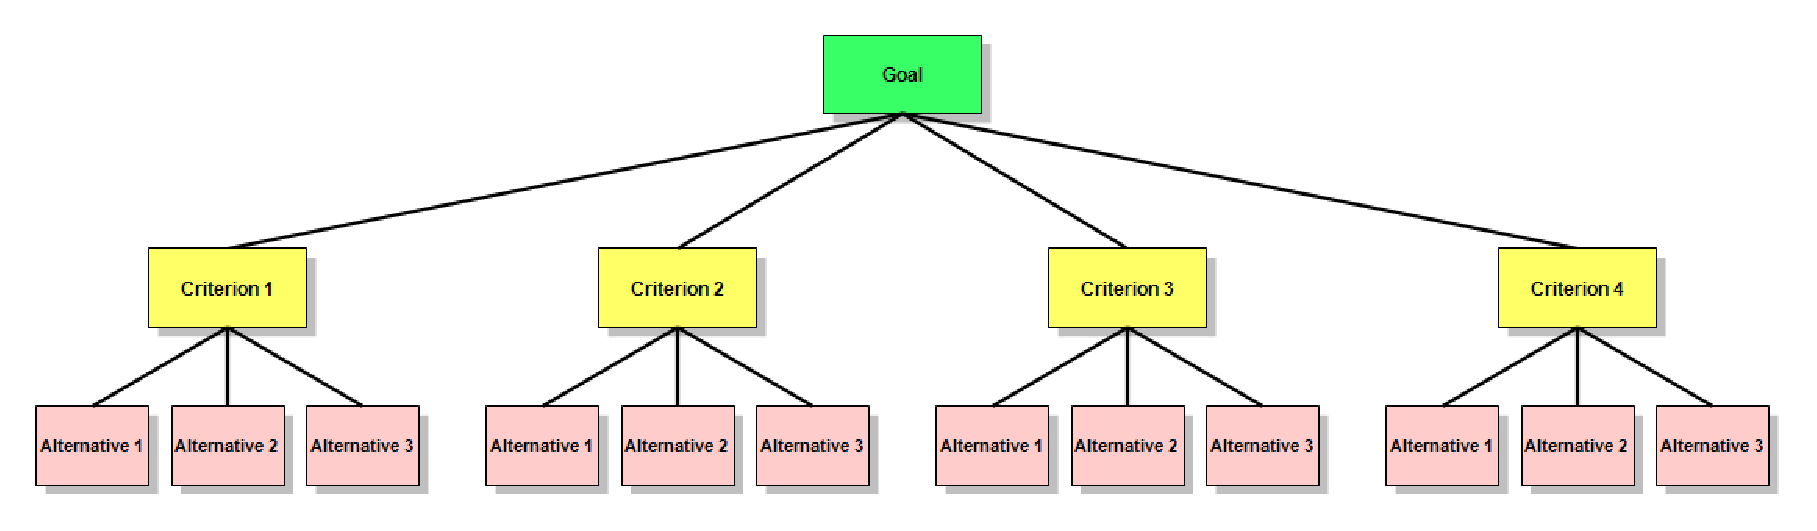
\includegraphics[width=16cm]{AHPHierarchy3.eps}
\caption{A simple AHP hierarchy}
\label{fig:graph}
\end{figure}

\subsection{Grey relational analysis model based on weighted entropy}

\par Grey relational analysis uses a specific concept of information. It defines situations with no information as black ,  and those with perfect information as white. However ,  neither of these idealized situations ever occurs in real world problems. In fact ,  situations between these extremes are described as being grey ,  hazy or fuzzy. Therefore ,  a grey system means that a system in which part of information is known and part of information is unknown. With this definition ,  information quantity and quality form a continuum from a total lack of information to complete information ? from black through grey to white. Since uncertainty always exists ,  one is always somewhere in the middle ,  somewhere between the extremes ,  somewhere in the grey area.
\par Grey analysis then comes to a clear set of statements about system solutions. At one extreme ,  no solution can be defined for a system with no information. At the other extreme ,  a system with perfect information has a unique solution. In the middle ,  grey systems will give a variety of available solutions. Grey analysis does not attempt to find the best solution ,  but does provide techniques for determining a good solution ,  an appropriate solution for real world problems.

\par In order to improve the low evaluation precision that the grey relational analysis method has been ,  the entropy theory was integrated to establish a new model.We use grey relational analysis model based on weighted entropy to judge the coaches' objective aspect.

\section{Model Establishment} 

\subsection{Objective Judgment Model----Using GRAP}
\par Because the analytic hierarchy process is influenced by the subjective factors ,  we use the grey relational model based on the entropy weight method to judge at the same time ,  and the results obtained by the two models are aggregated according to a certain weight.
\par We assume there have $n$ coaches and $m$ aspects of judgement , which formed the evaluation matrix. According to the assumptions , we have
\begin{equation}
X={({x}_{ij})}_{n\times m}
\end{equation}
where the matrix $X$ has been carried out after the standardized data.
\par In order to using the matrix above to solve , we have to figure out the information entropy of each index:

 \begin{equation}
 {E}_{j}=-\ln {{n}^{-1}} \sum_{i=1}^{n}{p}_{ij}\ln{ {p}_{ij}}
 \end{equation}
 
Where
\begin{equation}
{p}_{ij}={x}_{ij}/sum_{i=1}^{n}{x}_{ij}
\end{equation}
\par if~${p}_{ij}~=0$ , then define
\begin{equation}
\lim_{{p}_{ij}\rightarrow 0}{p}_{ij}\ln {{p}_{ij}}=0
\end{equation}
\par Whose solutions are${E}_{1} , {E}_{2} ,..., {E}_{k}$.The weight of each index is calculated by the information entropy:
\begin{equation}
{W}_{j}=\frac{1-{E}_{i}}{k-\sum{E}_{i}} ~~(i=1 , 2 ,..., k)
\end{equation}
\par Considering the limitations of the grey relational model ,  we combine the grey relational model with the information entropy to construct the grey relational model based on entropy weight method.In this model , we constitute a reference data column with the optimal value of each column:
\begin{equation}
{X}_{0}=({X}_{0}(1) ,  {X}_{0}(2) ,...,  {X}_{0}(n))
\end{equation}
\par Calculate the absolute difference between the target sequence and the reference sequence corresponding element of each evaluated object , which is
\begin{equation}
{\Delta }_{i}(j)=\mid {X}_{i}(j)-{X}_{0}(j)\mid ~~~j=1 , 2 ,..., n
\end{equation}
Where ${X}_{0}(j)$ represents the reference data of ${j}^{th}$ measurement criterion.
\par Using the data of Division one , we find the intermediate variables:
\begin{equation}
a=\min \limits_{1<i<n} \min \limits_{1<j<n}\{{\Delta }_{i}(j)\}
\end{equation}
\begin{equation}
b=\max \limits_{1<i<n} \max \limits_{1<j<n}\{{\Delta }_{i}(j)\}
\end{equation}
Calculated correlation coefficient:
\begin{equation}
{y}_{i}=\frac{a+b\rho }{{\Delta }_{i}(j)+b\rho }
\end{equation}
So that we can obtain the correlation degree:
\begin{equation}
{r}_{i}=\sum_{i=1}^{m}{W}_{j}{y}_{i}(j)~~~(i=1 , 2 ,.. .n)
\end{equation}
\par According to the correlation degree ,  we can calculate the final score and evaluate the coach.The results are followed:

\begin{figure}[!ht]
\centering
\includegraphics[width=12cm]{FootballResult.pdf}
\caption{Correlation Degree of Each Coach(Football)}
\label{fig:graph}
\end{figure}

\begin{figure} [!ht]
\centering
\includegraphics[width=12cm]{BaseballResult.pdf}
\caption{Correlation Degree of Each Coach(Baseball)}
\label{fig:graph}
\end{figure}

\begin{figure} [!ht]
\centering
\includegraphics[width=12cm]{BasketballResult.pdf}
\caption{Correlation Degree of Each Coach(Basketball)}
\label{fig:graph}
\end{figure}






\subsection{Subjective Judgment Model----Using AHP}
\par In an AHP hierarchy for college coach evolution ,  the goal might be to choose the best college coach or coaches (past or present) from among either male or female coaches in  football ,  baseball and basketball.The selection criteria might be decided by considering prestige ,  individual accolades  ,   winning rate , times of competition , times of winning champions and coaching time. Take those elements as six criterions.For this question , the alternatives might be those coaches.
\subsubsection{Constructing the Hierarchy}
\par As we  build our judging  hierarchy ,  the next step , we should investigate the values or measurements of the different elements that make it up. 
\par For the winning rate ,  times of competition ,  times of winning champions and coaching time ,  we can measure their importance through finding specific data. Because teams' participation in various sports leagues can best represent the level of coaching a team ,  we surf the MCAA's official website to gain the data as a standard to evaluate the elements. As for personal honor and prestige ,  we can't find the right data to measure. There are a thousand Hamlets in a thousand people's eyes ,  fans? evaluation of the coach will be interfered by the idea of the general public and some misleading informations.At this time ,  we can not take a quantitative way to measure him. Taking this factor into account ,  we use the number of Google searches to roughly measure the popularity of the coach. And the appropriate ratio is selected to be included in the analysis model of the whole hierarchy.

\subsubsection{Pairwise comparing the criteria with respect to the goal}
\par To incorporate their judgments about the various elements in the hierarchy ,  decision makers compare the elements two by two.  Right now ,  let's see which items are compared. Our example will begin with the six criteria in the second row of the hierarchy ,  though we could begin elsewhere if we wanted to. The criteria will be compared as to how important they are to the decision makers ,  with respect to the goal.Each pair of items in this row will be compared; there are a total of fifteen pairs.You can use the diagram below to see these pairs clearly.
\par Things change a bit when we get to the alternatives row. Here ,  the candidates in each group of alternatives are compared pair-by-pair with respect to the covering criterion of the group ,  which is the node directly above them in the hierarchy. What we are doing here is evaluating the models under consideration with respect to winning rate ,  then with respect to times of competition ,  then times of winning champions ,  coaching time ,  prestige ,  and individual accolades. Because there are $n$ coaches in the group of alternatives ,  there will be $\binom{n}{2}$ comparisons for each of the eight covering criteria.

\subsubsection{Making the decision}
\par On the basis of the last chapter ,  we construct the judgment matrix.Assuming a certain layer has $n$ factors , 
\begin{equation}
X={{x}_{1} , {x}_{2} ,..., {x}_{n}}
\end{equation}
\par To compare the upper layer of a certain criterion ,  we have to determine the proportion relative to a certain criterion.we define~${a}_{ij} $~to measure the comparison results of the ${i}^{th}$ factor relative to the ${j}^{th}$ factor , and we have:
\begin{equation}
{a}_{ij}=\frac{1}{{a}_{ij}}
\end{equation}
\begin{equation}
A={({a}_{ij})}_{n\times m}=
\begin{vmatrix}
{a}_{11} & {a}_{12} &... &{a}_{1n} \\ 
 {a}_{21}&{a}_{22}&...&{a}_{2n} \\ 
.. .&...  &...&... \\ 
 {a}_{n1}& {a}_{n2}&...&{a}_{nn} \\
\end{vmatrix}
\end{equation}
Where $n=6$.Meanwhile , the judgment matrix is obtained with the scale of $1-9$ as follows:
\begin{equation}
\begin{vmatrix}
 1& 3 &5  &5  &7  &9 \\ 
 \frac{1}{3}& 1 & 3 & 3 &5  &7 \\ 
 \frac{1}{5}&   \frac{1}{3}&  1&  3&  3&5 \\ 
 \frac{1}{5}&  \frac{1}{5} & \frac{1}{3}  &1  &  3&5 \\ 
 \frac{1}{7}&  \frac{1}{5} &   \frac{1}{5}&  \frac{1}{3} &  1& 3\\ 
 \frac{1}{9}&  \frac{1}{7} &  \frac{1}{5} &  \frac{1}{5} &  \frac{1}{3} & 1\\
\end{vmatrix}
\end{equation}
\par We define maximum eigenvalue of~$A$~is~${\lambda }_{max}$ , the corresponding feature vector is~${W}_{0}$~.We can obtain~$W$~after inputing normalized feature vector , which is the weight vector.
\begin{equation}
W=\frac{{\lambda }_{max}-n}{n-1}
\end{equation}
Calculating the coincidence indicator:
\begin{equation}
CI=\frac{{\lambda }_{max}-n}{n-1}
\end{equation}
Calculating the coincidence ratio:
\begin{equation}
CR=\frac{CI}{RI}
\end{equation}
\par When~$n=6$~ , the result of~$RI$~is~$1.24$~.After bringing data into model , we obtain~$CR=0.050262$~.The result of $CR$ is smaller than ~$0.1$~ , therefore , the consistency of judgment matrix is acceptable.


\begin{figure} [h]
\centering
\includegraphics[width=9cm]{Football.pdf}
\caption{ Evaluation Value of Each Coach(Football)}
\label{fig:graph}
\end{figure}

\begin{figure} [h]
\centering
\includegraphics[width=9cm]{Baseball.pdf}
\caption{Evaluation Value of Each Coach(Baseball)}
\label{fig:graph}
\end{figure}

\begin{figure} [h]
\centering
\includegraphics[width=9cm]{Basketball.pdf}
\caption{Evaluation Value of Each Coach(Basketball)}
\label{fig:graph}
\end{figure}

\subsection{The Influence  of other Factors}
\subsubsection{Time Influence}
\par Any kind of sport is constantly developing. The number of participants should  increase at first and then tends to be stable ,  it can be considered that the trend follows the logistic growth curve ,  the strength of the competition can also be reflected by the curve.
\par We define~${P}_{t}$~as the strength of competition , ~${P}_{t}$~has to take mean value standardization.~$S$~is the Integrated score of coaches.~$S'$~is the final score of coaches.
\begin{equation}
S'={P}_{t}S
\end{equation}
\par Time factor is too complex ,  in order to simplify the model ,  we have not taken it into account.
\subsubsection{ Sex Influence}
\par Considering the gender-specific sports have different ways of competitive , we find that the influence of sex is very small.So in this question , we would ignore it.
\section{Solving the Model} 
\par Because the analytic hierarchy process is influenced by the subjective factors ,  we use the grey relational model based on the entropy weight method to judge at the same time ,  and the results obtained by the two models are aggregated according to a certain weight.
\par We define the final score is~$S$~ , and the scale coefficients are~$\alpha $~(subjective coefficient)and~$\beta $~(objective coefficient).According to the models we have already built , we can obtain that:
\begin{equation}
S=\alpha r+\beta W
\end{equation}
Where ~$\alpha $~ is taking 0.4 and ~$\beta $~is taking 0.6.
\par After taking the data we solve above into calculating , we can gain the final result as follows:

\begin{table}[h]
\centering
 \caption{\label{tab:test}Top 5 Coaches of Football}
 \begin{tabular}{ccccc}
  \toprule
 No.1 & No.2 & No.3 & No.4 & No.5 \\
  \midrule
Ron Schipper  & Larry Kehres & Mike Kelly &Tom Osborne&Fielding Yost \\
Hope &Mount Union &Manchester&Hastings&West Virginia\\
  \bottomrule
 \end{tabular}
\end{table}


\begin{table}[h]
\centering
 \caption{\label{tab:test}Top 5 Coaches of Basetball}
 \begin{tabular}{ccccc}
  \toprule
 No.1 & No.2 & No.3 & No.4 & No.5 \\
  \midrule
Gene Stephenson  & Mike Martin & Don Schaly &Cliff Gustafson&Frank Vieira \\
Wichita St. &Florida St.  &Marietta &Texas&New Haven \\
  \bottomrule
 \end{tabular}
\end{table}

\begin{table}[!ht]
\centering
 \caption{\label{tab:test}Top 5 Coaches of Basketball}
 \begin{tabular}{ccccc}
  \toprule
 No.1 & No.2 & No.3 & No.4 & No.5 \\
  \midrule
Adolph Rupp  & Dean Smith & Jerry Tarkanian &Dave Robbins&John Wooden \\
Kentucky &North Carolina &Fresno St. &Virginia Union&UCLA\\
  \bottomrule
 \end{tabular}
\end{table}

\par This result is in good agreement with the objective evaluation model ,  which is compared with the model we have constructed.So the choice of ratio coefficient is very scientific.

\section{Strengths and Weaknesses}

\subsection{Strengths}
\par Our model effectively achieves all of the goals we set initially. It is fast and can handle large quantities data of coaches performance , but also have the flexibility we desired.Though we did not test all kinds of ball games and all the college coaches , we showed that our model optimizes state districts for any of a number of variables.Our model can rank the coaches from past to current , it has wide range of application and good time applicability.As well , our method is robust.

\subsection{Weaknesses}
\par Weakness of the model included assumptions made for simplicity that likely do not hold.And some special data can't be found , and it makes that we have to do some proper assumption before the solution of our models.For instance , we can't the data of the coaches' popularity , so we take  Google search volume as an alternative.A more abundant data resource can guarantee a better result in our models.


\section{the Article for Sports Illustrated}
\begin{center}
\textbf{\Large{\emph{Cream of The Crop----Looking for The Best All Time College Coach}}}
\end{center}
\par Measurement implies difference. When you measure ,  you take the difference between the starting point and the finishing point. Then you can see the difference change.Difference is not necessarily of value. It has to be put into context to see what it means. It needs to be measured against some other coaches to provide the context ,  and then it can be evaluated.Evaluation adds meaning to measurement.
\par Different people have different measurement standards.People born to be biased to their own preference.People may prefer those teams , which are related to him.If I live in New York City , the New York Yankees might
be my favorite team.However , ranking isn't always follow our own hearts.After reference to various data about college coaches from MACC , we can put forward an undisputed ranking.Here are the top 5 greatest college coaches over the course of sports history in football , baseball and basketball as follows:
\begin{table}[h]
\centering
 \caption{\label{tab:test}Top 5 Coaches}
 \begin{tabular}{ccccc}
  \toprule
 No.1 & No.2 & No.3 & No.4 & No.5 \\
  \midrule
 &&Football&&\\
 \hline
Ron Schipper  & Larry Kehres & Mike Kelly &Tom Osborne&Fielding Yost \\
Hope &Mount Union &Manchester&Hastings&West Virginia\\
\hline
&&Baseball&&\\
\hline
Gene Stephenson  & Mike Martin & Don Schaly &Cliff Gustafson&Frank Vieira \\
Wichita St. &Florida St.  &Marietta &Texas&New Haven \\
\hline
&&Basketball&&\\
\hline
Adolph Rupp  & Dean Smith & Jerry Tarkanian &Dave Robbins&John Wooden \\
Kentucky &North Carolina &Fresno St. &Virginia Union&UCLA\\
  \bottomrule
 \end{tabular}
\end{table}
\par Ron Schipper  ,  the highest ranking coach.who had 36 years coaching experience.During his coaching life , he won 3 national championships.The win-loss record is 287-67 and winning-percentage is 0.808 , the highest in NCAA.Take various factors into consideration  , there is no doubt that Ron was the greatest college football coach.We appreciate this honorable coach , he not only help his own team became the most shining  team in NCAA , but also promote the development of Football.
\par College sports are various , the number of coaches is enormous.The method we took is balance the factors of subjectivity and objectivity.If you have interest in our way to evaluate your own favorite coach  , please contract us.Whether you have enough data or not  , our model would always get the your own answer.


\begin{thebibliography}{99}
\bibitem{1} D.~E. KNUTH   The \TeX{}book  the American
Mathematical Society and Addison-Wesley
Publishing Company  ,  1984-1986.
\bibitem{2}Lamport ,  Leslie ,   \LaTeX{}: `` A Document Preparation System '' , 
Addison-Wesley Publishing Company ,  1986.
\bibitem{3}Al-Harbi ,  Al Subhi ,  Application of the AHP in project management. Int J Proj Manag , 
International Journal of Project Management ,  2001.
\bibitem{4}\url{https://en.wikipedia.org/wiki/Analytic_hierarchy_process_?_car_example#Pairwise_comparing_the_criteria_with_respect_to_the_goal}
\bibitem{5}Guo liang ,  L. I. and Qiang ,  F. U. and Sun ,  Yong and Feng ,  Yan ,  Grey relational analysis model based on weighted entropy and its Application , 
Journal of Water Resources and Water Engineering ,  2006.
\end{thebibliography}

\begin{appendices}
\section{The Data of Objective Judgement Model}
\par Here are the final score of coaches we  calculated in our model as follow.
\begin{longtable}{ccc}
 &Table A1:The Result of Football Coach Ranking&\\
 \hline
Final Rank & Coach Name & Score\\
\hline
\endhead

1     & 25. Ron Schipper (Hope 1952 & 0.861323 \\
    2     & 1. Larry Kehres (Mount Union 1971 & 0.828949 \\
    3     & 19. Mike Kelly (Manchester 1970 & 0.61444 \\
    4     & 11. Tom Osborne (Hastings 1959 & 0.606615 \\
    5     & 14. Fielding Yost (West Virginia 1895 & 0.596344 \\
    6     & 8. Jake Gaither (Knoxville 1927 & 0.538745 \\
    7     & 27. Chuck Broyles (Pittsburg St. 1970 & 0.490908 \\
    8     & 20. Henry A. Kean (Fisk 1920 & 0.485191 \\
    9     & 16. Bob Neyland (Army 1916 & 0.47542 \\
    10    & 23. Jock Sutherland (Pittsburgh 1918 & 0.44586 \\
    11    & 22. *Joe Fincham (Ohio 1988 & 0.433482 \\
    12    & 10. Barry Switzer (Arkansas 1960 & 0.430033 \\
    13    & 17. Bud Wilkinson (Minnesota 1937 & 0.427063 \\
    14    & 4. Bob Reade (Cornell College 1954 & 0.422136 \\
    15    & 24. *Pete Fredenburg (Texas St. 1970 & 0.416481 \\
    16    & 26. Bob Devaney (Alma 1939 & 0.415111 \\
    17    & 6. Dick Farley (Boston U. 1968 & 0.407455 \\
    18    & 18. Chuck Klausing (Slippery Rock 1948 & 0.406921 \\
    19    & 9. Dave Maurer (Denison 1954 & 0.405277 \\
    20    & 13. Don Coryell (Washington 1950 & 0.403988 \\
    21    & 7. George Woodruff (Yale 1889 & 0.399163 \\
    22    & 3. Frank Leahy (Notre Dame 1931 & 0.382276 \\
    23    & 2. Knute Rockne (Notre Dame 1914 & 0.381243 \\
    24    & 12. *Urban Meyer (Cincinnati 1986 & 0.378251 \\
    25    & 15  Percy Haughton (Harvard 1899 & 0.376209 \\
    26    & 21. *Mike Sirianni (Mount Union 1994 & 0.361356 \\
    27    & 29. Sid Gillman (Ohio St. 1934 & 0.355325 \\
    28    & 5. Doyt Perry (Bowling Green 1932 & 0.353612 \\
    29    & 28. Biggie Munn (Minnesota 1932 & 0.350625 \\
\end{longtable}


\begin{longtable}{ccc}
 &Table A2:The Result of Baseball Coach Ranking&\\
 \hline
Final Rank & Coach Name & Score\\
\hline
\endhead
% header ------------------------
1     & 24. *Gene Stephenson (Wichita St. 1978-10 & 0.90323638 \\
    2     & 21. *Mike Martin (Florida St. 1980-10 & 0.821028243 \\
    3     & 2. Don Schaly (Marietta 1964-03 & 0.783913293 \\
    4     & 8. Frank Vieira (New Haven 1963-06 & 0.717971261 \\
    5     & 4. Cliff Gustafson (Texas 1968-96 & 0.703452693 \\
    6     & 28. Ron Fraser (Miami [FL] 1963-92 & 0.646819868 \\
    7     & 23. *Mike Fox (N.C. Wesleyan 1983-94 ,  96-98 ,  & 0.576177312 \\
    8     & 3. John Barry (Holy Cross 1921-60 & 0.571706219 \\
    9     & 26. *Bob Babb (Johns Hopkins 1980-10 & 0.555972193 \\
    10    & 29. G ary Ward (Oklahoma St. 1978-96 ,  & 0.538544621 \\
    11    & 20. Frank Sancet (Arizona 1950-72 & 0.505388576 \\
    12    & 10. Chuck Anderson (Fla. Southern 1967 ,  & 0.4969309 \\
    13    & 30. W.J. Disch (Texas 1911-39 & 0.481050838 \\
    14    & 25. Bob Wren (Ohio 1949-72 & 0.452256656 \\
    15    & 9. *Mike Kinnison (Delta St. 1997-10 & 0.441752081 \\
    16    & 14. G eorge Huff (Illinois 1896-19 & 0.434465608 \\
    17    & 11. Dennis Denning (St. Thomas [MN] 1995-09 & 0.429926877 \\
    18    & 17. Bobby Winkles (Arizona St. 1959-71 & 0.424797585 \\
    19    & 22. Chase Riddle (Troy 1979-90 & 0.41053337 \\
    20    & 7. Russ Tiedmann (Wis.-Oshkosh 1975-88 & 0.407563437 \\
    21    & 13. *Joe Urso (Tampa 2001-10 & 0.407090652 \\
    22    & 6. *Joe Brown (SUNY Cortland 2000-10 & 0.404193028 \\
    23    & 18. *James Vilade (Dallas 1998-01 ,  & 0.397783307 \\
    24    & 16. H arry Carlson (Springfield 1924 ,  & 0.396234266 \\
    25    & 15. *Doug Fleetwood (Salisbury 2001-10 & 0.394269781 \\
    26    & 19. Carleton Wood (St. Bonaventure 1951 ,  & 0.39328301 \\
    27    & 5. Mark Walsh (Aurora 1993-02 & 0.392276822 \\
    28    & 1. Robert Henry Lee (Southern U. 1949-60 & 0.381618164 \\
    29    & 27. G eorge Jacobs (Villanova 1933-43 & 0.372694559 \\
    30    & 12. William Spaulding (Western Mich. 1911-21 & 0.368779134 \\
\end{longtable}



\begin{longtable}{ccc}
 &Table A3:The Result of Basketball Coach Ranking&\\
 \hline
Final Rank & Coach Name & Score\\
\hline
\endhead
% header ------------------------
1     & 2. Adolph Rupp  Kentucky 1931-52 ,  54-72 & 0.995112 \\
    2     & 12. Dean Smith North Carolina 1962-97 & 0.897544 \\
    3     & 10. Jerry Tarkanian Long Beach St.1969-73 ,  UNLV 74-92& 0.662902 \\
    4     & 9. Dave Robbins Virginia Union 1979-2008 & 0.640727 \\
    5     & 5. John Wooden Indiana St. 1947-48 , UCLA 49-75  & 0.598213 \\
    6     & 16. Steve Moore  Muhlenberg 1982-87 , Wooster 88-2010* & 0.575382 \\
    7     & 29. Dean Nicholson Central Wash. 1965-90  & 0.548798 \\
    8     & 18. Bo Ryan Wis.-Platteville 1985-99 , Wisconsin 02-10*  & 0.538454 \\
    9     & 7. Roy Williams Kansas 1989-2003 , North Carolina 04-10* & 0.52028 \\
    10    & 28. Ron Niekamp  Findlay 1986-2010* & 0.514847 \\
    11    & 8. John KresseCol. of Charleston 1980-2002 & 0.500042 \\
    12    & 19. Frank M. Keaney Rhode Island 1921-48 & 0.478122 \\
    13    & 20. George Keogan Allegheny 19 ,  Notre  Dame 24-43\#  & 0.473997 \\
    14    & 13. Ed AdamsN.C. Central 1937 , Texas Southern 50-58 & 0.457006 \\
    15    & 1. Clair Bee Rider 1929-31 , Long Island 32-43 ,  46-51 & 0.435227 \\
    16    & 14. Bruce PearlSouthern Ind.1993-2001 ,  Tennessee 06-10* & 0.429834 \\
    17    & 30. Harry Sheehy (Williams 1975) Williams 1984-2000  & 0.392285 \\
    18    & 22. Mike Jones 1989-2002 ,  07-08 & 0.389534 \\
    19    & 23. Lucias Mitchell AlabamaNorfolk St. 79-81 & 0.384299 \\
    20    & 26. Jim Borcherding (Wartburg 1962)Augustana (IL) 1970-84 & 0.381434 \\
    21    & 27. Mike DunlapCal Lutheran 1990-94 ,  Metro St. 98-2006 & 0.381194 \\
    22    & 15. Charles Christian Norfolk St. 1974-78 ,  82-90 & 0.378824 \\
    23    & 11. Francis Schmidt Tulsa 1916-17 ,  19-22 , Arkansas 24-29 ,   & 0.377533 \\
    24    & 6. Mark Few (Oregon 1987) Gonzaga 2000-10* & 0.362184 \\
    25    & 24. Harry Fisher  Columbia07-16 ,  Army 07 ,  22-23 ,  25  & 0.359765 \\
    26    & 25. Ed Green (Clarion 1964) Roanoke 1978-89 & 0.358666 \\
    27    & 3. Walter Bucky HarrisPhiladelphia U. 1954-65 ,  67 & 0.358211 \\
    28    & 4. Dolph Stanley ( Beloit 1946-57 & 0.354311 \\
    29    & 17. Jack Ramsay (St. Joseph��s 1949) St. Joseph��s 1956-66  & 0.349427 \\
    30    & 21. Vic Bubas (North Carolina St. 1951) Duke 1960-69  & 0.342712 \\
\end{longtable}

\section{The Data of Subjective Judgement Model }

\begin{longtable}{ccc}
 &Table A4:The Result of Football Coach Ranking&\\
 \hline
Final Rank & Coach Name & Evaluation Value\\
\hline
\endhead

 1     & 1. Larry Kehres (Mount Union 1971 & 1.12755 \\
    2     & 25. Ron Schipper (Hope 1952 & 1.108272 \\
    3     & 11. Tom Osborne (Hastings 1959 & 0.997158 \\
    4     & 19. Mike Kelly (Manchester 1970 & 0.993665 \\
    5     & 14. Fielding Yost (West Virginia 1895 & 0.930321 \\
    6     & 8. Jake Gaither (Knoxville 1927 & 0.91647 \\
    7     & 27. Chuck Broyles (Pittsburg St. 1970 & 0.875636 \\
    8     & 16. Bob Neyland (Army 1916 & 0.84018 \\
    9     & 20. Henry A. Kean (Fisk 1920 & 0.837924 \\
    10    & 10. Barry Switzer (Arkansas 1960 & 0.793259 \\
    11    & 22. *Joe Fincham (Ohio 1988 & 0.790624 \\
    12    & 4. Bob Reade (Cornell College 1954 & 0.784771 \\
    13    & 23. Jock Sutherland (Pittsburgh 1918 & 0.783374 \\
    14    & 17. Bud Wilkinson (Minnesota 1937 & 0.777045 \\
    15    & 24. *Pete Fredenburg (Texas St. 1970 & 0.765534 \\
    16    & 7. George Woodruff (Yale 1889 & 0.751132 \\
    17    & 26. Bob Devaney (Alma 1939 & 0.750005 \\
    18    & 9. Dave Maurer (Denison 1954 & 0.74595 \\
    19    & 13. Don Coryell (Washington 1950 & 0.740235 \\
    20    & 6. Dick Farley (Boston U. 1968 & 0.736036 \\
    21    & 18. Chuck Klausing (Slippery Rock 1948 & 0.736011 \\
    22    & 2. Knute Rockne (Notre Dame 1914 & 0.710502 \\
    23    & 3. Frank Leahy (Notre Dame 1931 & 0.705068 \\
    24    & 12. *Urban Meyer (Cincinnati 1986 & 0.702866 \\
    25    & 15  Percy Haughton (Harvard 1899 & 0.678282 \\
    26    & 21. *Mike Sirianni (Mount Union 1994 & 0.654123 \\
    27    & 5. Doyt Perry (Bowling Green 1932 & 0.641562 \\
    28    & 29. Sid Gillman (Ohio St. 1934 & 0.629187 \\
    29    & 28. Biggie Munn (Minnesota 1932 & 0.61327 \\
 \end{longtable}


\begin{longtable}{ccc}
 &Table A5:The Result of Baseball Coach Ranking&\\
 \hline
Final Rank & Coach Name & Evaluation Value\\
\hline
\endhead
% header ------------------------
1     & 24. *Gene Stephenson (Wichita St. 1978-10 & 1.228556 \\
    2     & 21. *Mike Martin (Florida St. 1980-10 & 1.183313 \\
    3     & 2. Don Schaly (Marietta 1964-03 & 1.153538 \\
    4     & 4. Cliff Gustafson (Texas 1968-96 & 1.098829 \\
    5     & 8. Frank Vieira (New Haven 1963-06 & 1.065278 \\
    6     & 28. Ron Fraser (Miami [FL] 1963-92 & 1.047706 \\
    7     & 23. *Mike Fox (N.C. Wesleyan 1983-94 ,  96-98 ,  & 0.964883 \\
    8     & 26. *Bob Babb (Johns Hopkins 1980-10 & 0.918692 \\
    9     & 29. G ary Ward (Oklahoma St. 1978-96 ,  & 0.91678 \\
    10    & 3. John Barry (Holy Cross 1921-60 & 0.879881 \\
    11    & 20. Frank Sancet (Arizona 1950-72 & 0.856509 \\
    12    & 10. Chuck Anderson (Fla. Southern 1967 ,  & 0.852685 \\
    13    & 30. W.J. Disch (Texas 1911-39 & 0.766118 \\
    14    & 9. *Mike Kinnison (Delta St. 1997-10 & 0.749163 \\
    15    & 25. Bob Wren (Ohio 1949-72 & 0.727642 \\
    16    & 11. Dennis Denning (St. Thomas [MN] 1995-09 & 0.715938 \\
    17    & 17. Bobby Winkles (Arizona St. 1959-71 & 0.701791 \\
    18    & 14. G eorge Huff (Illinois 1896-19 & 0.683349 \\
    19    & 13. *Joe Urso (Tampa 2001-10 & 0.663881 \\
    20    & 22. Chase Riddle (Troy 1979-90 & 0.661495 \\
    21    & 6. *Joe Brown (SUNY Cortland 2000-10 & 0.660434 \\
    22    & 7. Russ Tiedmann (Wis.-Oshkosh 1975-88 & 0.65988 \\
    23    & 5. Mark Walsh (Aurora 1993-02 & 0.631117 \\
    24    & 18. *James Vilade (Dallas 1998-01 ,  & 0.627339 \\
    25    & 15. *Doug Fleetwood (Salisbury 2001-10 & 0.622995 \\
    26    & 1. Robert Henry Lee (Southern U. 1949-60 & 0.612291 \\
    27    & 19. Carleton Wood (St. Bonaventure 1951 ,  & 0.600229 \\
    28    & 16. H arry Carlson (Springfield 1924 ,  & 0.592802 \\
    29    & 27. G eorge Jacobs (Villanova 1933-43 & 0.536152 \\
    30    & 12. William Spaulding (Western Mich. 1911-21 & 0.533849 \\
\end{longtable}



\begin{longtable}{ccc}
 &Table A6:The Result of Basketball Coach Ranking&\\
 \hline
Final Rank & Coach Name & Evaluation Value\\
\hline
\endhead
% header ------------------------
1     & 2. Adolph Rupp (Kansas 1923) Kentucky 1931-52 ,  54-72 & 1.122933 \\
    2     & 12. Dean Smith (Kansas 1953) North Carolina 1962-97 & 1.100008 \\
    3     & 10. Jerry TarkanianUNLV 74-92 ,  Fresno St. 96-2002  & 0.996622 \\
    4     & 9. Dave RobbinsVirginia Union 1979-2008 & 0.983505 \\
    5     & 5. John Wooden Indiana St. 1947-48 , UCLA 49-75  & 0.955703 \\
    6     & 16. Steve Moore Muhlenberg 1982-87 , Wooster 88-2010* & 0.929097 \\
    7     & 29. Dean Nicholson Central Wash. 1965-90  & 0.910848 \\
    8     & 18. Bo Ryan Milwaukee 2000-01 ,  Wisconsin 02-10*  & 0.900834 \\
    9     & 7. Roy Williams  Kansas 1989-2003 , North Carolina 04-10* & 0.895349 \\
    10    & 28. Ron Niekamp  Findlay 1986-2010* & 0.875743 \\
    11    & 8. John Kresse Col. of Charleston 1980-2002 & 0.872021 \\
    12    & 13. Ed Adams Tuskegee 38-49 ,  Texas Southern 50-58 & 0.811021 \\
    13    & 20. George Keogan (Minnesota ) Wis.-Superior 1913-14& 0.804024 \\
    14    & 19. Frank M. Keaney (Bates 1911) Rhode Island 1921-48 & 0.802093 \\
    15    & 1. Clair Bee (Clair Bee Rider 1929-31 , 46-51 & 0.794039 \\
    16    & 14. Bruce PearlTennessee 06-10* & 0.780112 \\
    17    & 30. Harry Sheehy Williams 1984-2000  & 0.705595 \\
    18    & 22. Mike Jones 1975)Mississippi Col. 1989-2002 ,  07-08 & 0.705137 \\
    19    & 23. Lucias Mitchell Alabama St. 1964-67 ,  Norfolk St. 79-81 & 0.697322 \\
    20    & 27. Mike Dunlap Cal Lutheran 1990-94 ,  Metro St. 98-2006 & 0.694085 \\
    21    & 15. Charles Christian Norfolk St. 1974-78 ,  82-90 & 0.69285 \\
    22    & 26. Jim Borcherding Augustana (IL) 1970-84 & 0.690489 \\
    23    & 11. Francis Schmidt Tulsa 1916-17 ,   TCU 30-34 & 0.67958 \\
    24    & 6. Mark Few (Oregon 1987) Gonzaga 2000-10* & 0.675407 \\
    25    & 3. Walter Bucky Harris Philadelphia U. 1954-65 ,  67 & 0.663652 \\
    26    & 4. Dolph Stanley  Beloit 1946-57 & 0.657502 \\
    27    & 25. Ed Green (Clarion 1964) Roanoke 1978-89 & 0.647179 \\
    28    & 17. Jack Ramsay  St. Joseph��s 1956-66  & 0.629524 \\
    29    & 24. Harry Fisher Fordham 1905 ,   Army 07 ,  22-23 ,  25  & 0.627561 \\
    30    & 21. Vic Bubas (North Carolina St. 1951) Duke 1960-69  & 0.61328 \\
\end{longtable}
\end{appendices}

\end{document}
